\documentclass{beamer}
\usetheme{Madrid}
\definecolor{oucrimson}{RGB}{132,22,23}
\usecolortheme[named=oucrimson]{structure}

\usepackage{graphicx}
\usepackage{booktabs}
\usepackage{tikz}
\usetikzlibrary{positioning, arrows.meta, shapes.geometric}

\title[Income Shifting by MNEs]{What Drives Income Shifting by Multinational Enterprises?}
\author{Brent Myers}
\institute[University of Oklahoma]{University of Oklahoma \\ Econ 5253: Data Science for Economists}
\date{April 30, 2026}

\begin{document}

% ============================================================
% TITLE SLIDE
% ============================================================
\begin{frame}
\titlepage
\end{frame}

% ============================================================
% INTRO SLIDE 1: Income Shifting - Example 1
% ============================================================
\begin{frame}{Introduction}
\centerline{\large\textbf{Income Shifting -- Example 1}}
\vspace{0.1cm}
\centering
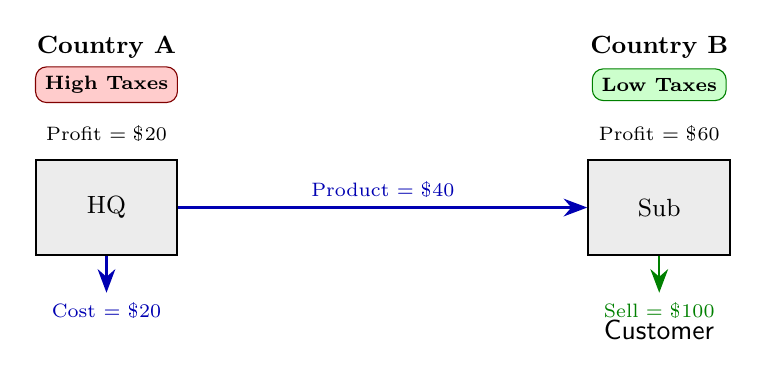
\begin{tikzpicture}[
  scale=0.78,
  box/.style={draw, thick, minimum width=1.8cm, minimum height=1.2cm, align=center, font=\small},
  label/.style={font=\small\bfseries},
  arrow/.style={-{Stealth[length=3mm]}, thick}
]
  % Country A (left side)
  \node[label] at (-4.5, 3.8) {Country A};
  \node[fill=red!20, draw=red!50!black, rounded corners, font=\scriptsize\bfseries] at (-4.5, 3.2) {High Taxes};

  % HQ building
  \node[box, fill=gray!15] (hq) at (-4.5, 1.2) {HQ};
  \node[font=\scriptsize, above=0.1cm of hq] {Profit = \$20};

  % Country B (right side)
  \node[label] at (4.5, 3.8) {Country B};
  \node[fill=green!20, draw=green!50!black, rounded corners, font=\scriptsize\bfseries] at (4.5, 3.2) {Low Taxes};

  % Subsidiary building
  \node[box, fill=gray!15] (sub) at (4.5, 1.2) {Sub};
  \node[font=\scriptsize, above=0.1cm of sub] {Profit = \$60};

  % Flow arrows
  \draw[arrow, blue!70!black] (hq.south) -- ++(0,-0.6) node[font=\scriptsize, below] {Cost = \$20};
  \draw[arrow, blue!70!black] (hq.east) -- node[above, font=\scriptsize] {Product = \$40} (sub.west);
  \draw[arrow, green!50!black] (sub.south) -- ++(0,-0.6) node[font=\scriptsize, below] {Sell = \$100};

  % Customer label (unbolded, moved closer to Sell)
  \node[font=\normalsize] at (4.5, -0.8) {\textsf{Customer}};
\end{tikzpicture}

\vspace{0.2cm}
{\small \textit{HQ sells product to subsidiary at a low transfer price (\$40), shifting \$60 of profit to the low-tax jurisdiction.}}
\end{frame}

% ============================================================
% INTRO SLIDE 2: Income Shifting - Example 2
% ============================================================
\begin{frame}{Introduction -- continued}
\centerline{\large\textbf{Income Shifting -- Example 2}}
\vspace{0.1cm}
\centering
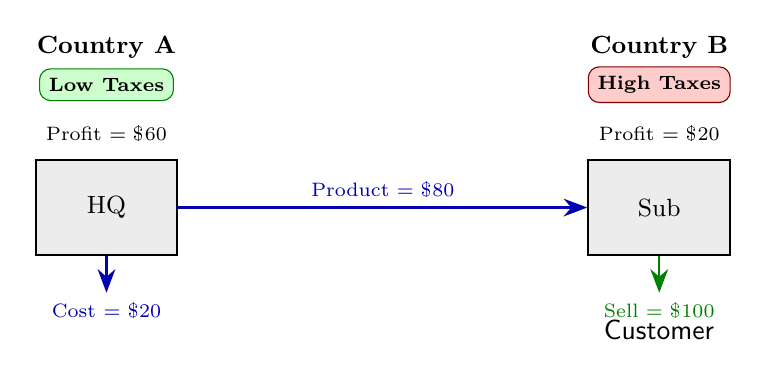
\begin{tikzpicture}[
  scale=0.78,
  box/.style={draw, thick, minimum width=1.8cm, minimum height=1.2cm, align=center, font=\small},
  label/.style={font=\small\bfseries},
  arrow/.style={-{Stealth[length=3mm]}, thick}
]
  % Country A (left side)
  \node[label] at (-4.5, 3.8) {Country A};
  \node[fill=green!20, draw=green!50!black, rounded corners, font=\scriptsize\bfseries] at (-4.5, 3.2) {Low Taxes};

  % HQ building
  \node[box, fill=gray!15] (hq) at (-4.5, 1.2) {HQ};
  \node[font=\scriptsize, above=0.1cm of hq] {Profit = \$60};

  % Country B (right side)
  \node[label] at (4.5, 3.8) {Country B};
  \node[fill=red!20, draw=red!50!black, rounded corners, font=\scriptsize\bfseries] at (4.5, 3.2) {High Taxes};

  % Subsidiary building
  \node[box, fill=gray!15] (sub) at (4.5, 1.2) {Sub};
  \node[font=\scriptsize, above=0.1cm of sub] {Profit = \$20};

  % Flow arrows
  \draw[arrow, blue!70!black] (hq.south) -- ++(0,-0.6) node[font=\scriptsize, below] {Cost = \$20};
  \draw[arrow, blue!70!black] (hq.east) -- node[above, font=\scriptsize] {Product = \$80} (sub.west);
  \draw[arrow, green!50!black] (sub.south) -- ++(0,-0.6) node[font=\scriptsize, below] {Sell = \$100};

  % Customer label (unbolded, moved closer to Sell)
  \node[font=\normalsize] at (4.5, -0.8) {\textsf{Customer}};
\end{tikzpicture}

\vspace{0.2cm}
{\small \textit{HQ raises the transfer price to \$80, keeping \$60 of profit in the low-tax jurisdiction.}}
\end{frame}

% ============================================================
% INTRO SLIDE 3: What is Income Shifting? (moved from old slide 2)
% ============================================================
\begin{frame}{Introduction -- continued}
\centerline{\large\textbf{What is Income Shifting?}}
\vspace{0.3cm}
\centering
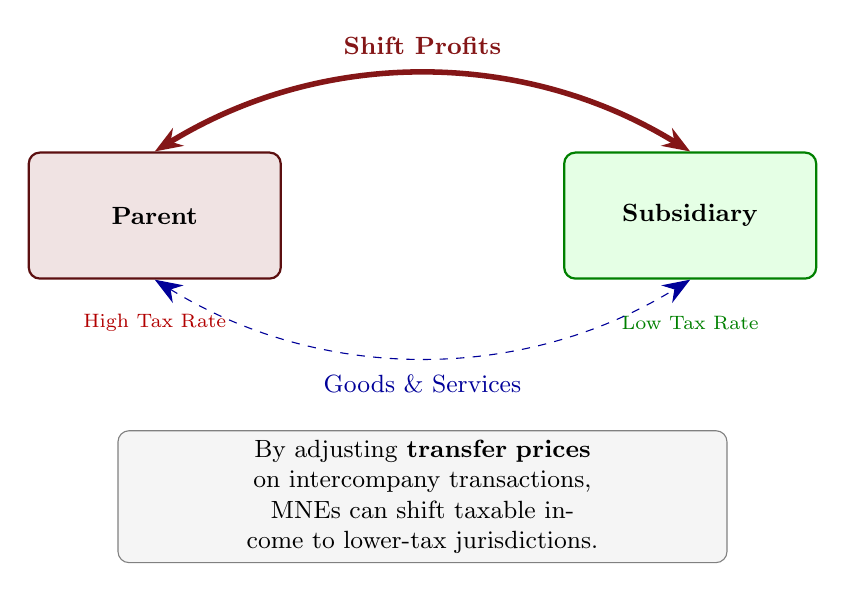
\begin{tikzpicture}[
  scale=0.85,
  entity/.style={draw, thick, rounded corners=4pt, minimum width=3.2cm, minimum height=1.6cm, align=center, font=\small},
  arrow/.style={-{Stealth[length=3.5mm]}, thick}
]
  % Parent box (no U.S. label)
  \node[entity, fill=oucrimson!12, draw=oucrimson!70!black] (parent) at (-4, 0) {\textbf{Parent}};

  % Subsidiary box (no Foreign label)
  \node[entity, fill=green!10, draw=green!50!black] (sub) at (4, 0) {\textbf{Subsidiary}};

  % Profit shifting arrow (bidirectional, curved, on top, no $ signs)
  \draw[{Stealth[length=3.5mm]}-{Stealth[length=3.5mm]}, oucrimson, line width=2pt] 
    (parent.north) .. controls (-1.5, 2.5) and (1.5, 2.5) .. (sub.north)
    node[midway, above=0.1cm, font=\small\bfseries] {Shift Profits};

  % Tax labels below boxes
  \node[font=\scriptsize, color=red!70!black] at (-4, -1.6) {High Tax Rate};
  \node[font=\scriptsize, color=green!50!black] at (4, -1.6) {Low Tax Rate};

  % Goods/services arrow (bidirectional, bottom)
  \draw[{Stealth[length=3.5mm]}-{Stealth[length=3.5mm]}, blue!60!black, dashed] 
    (parent.south) .. controls (-1.5, -2.5) and (1.5, -2.5) .. (sub.south)
    node[midway, below=0.1cm, font=\small] {Goods \& Services};

  % Result annotation
  \node[draw=gray, rounded corners, fill=gray!8, font=\small, text width=7.5cm, align=center] at (0, -4.2) {
    By adjusting \textbf{transfer prices} on intercompany transactions,\\
    MNEs can shift taxable income to lower-tax jurisdictions.
  };
\end{tikzpicture}
\end{frame}

% ============================================================
% INTRO SLIDE 4: Why Should We Care?
% ============================================================
\begin{frame}{Introduction -- continued}
\centerline{\large\textbf{Why Should We Care?}}
\vspace{0.1cm}
\centering
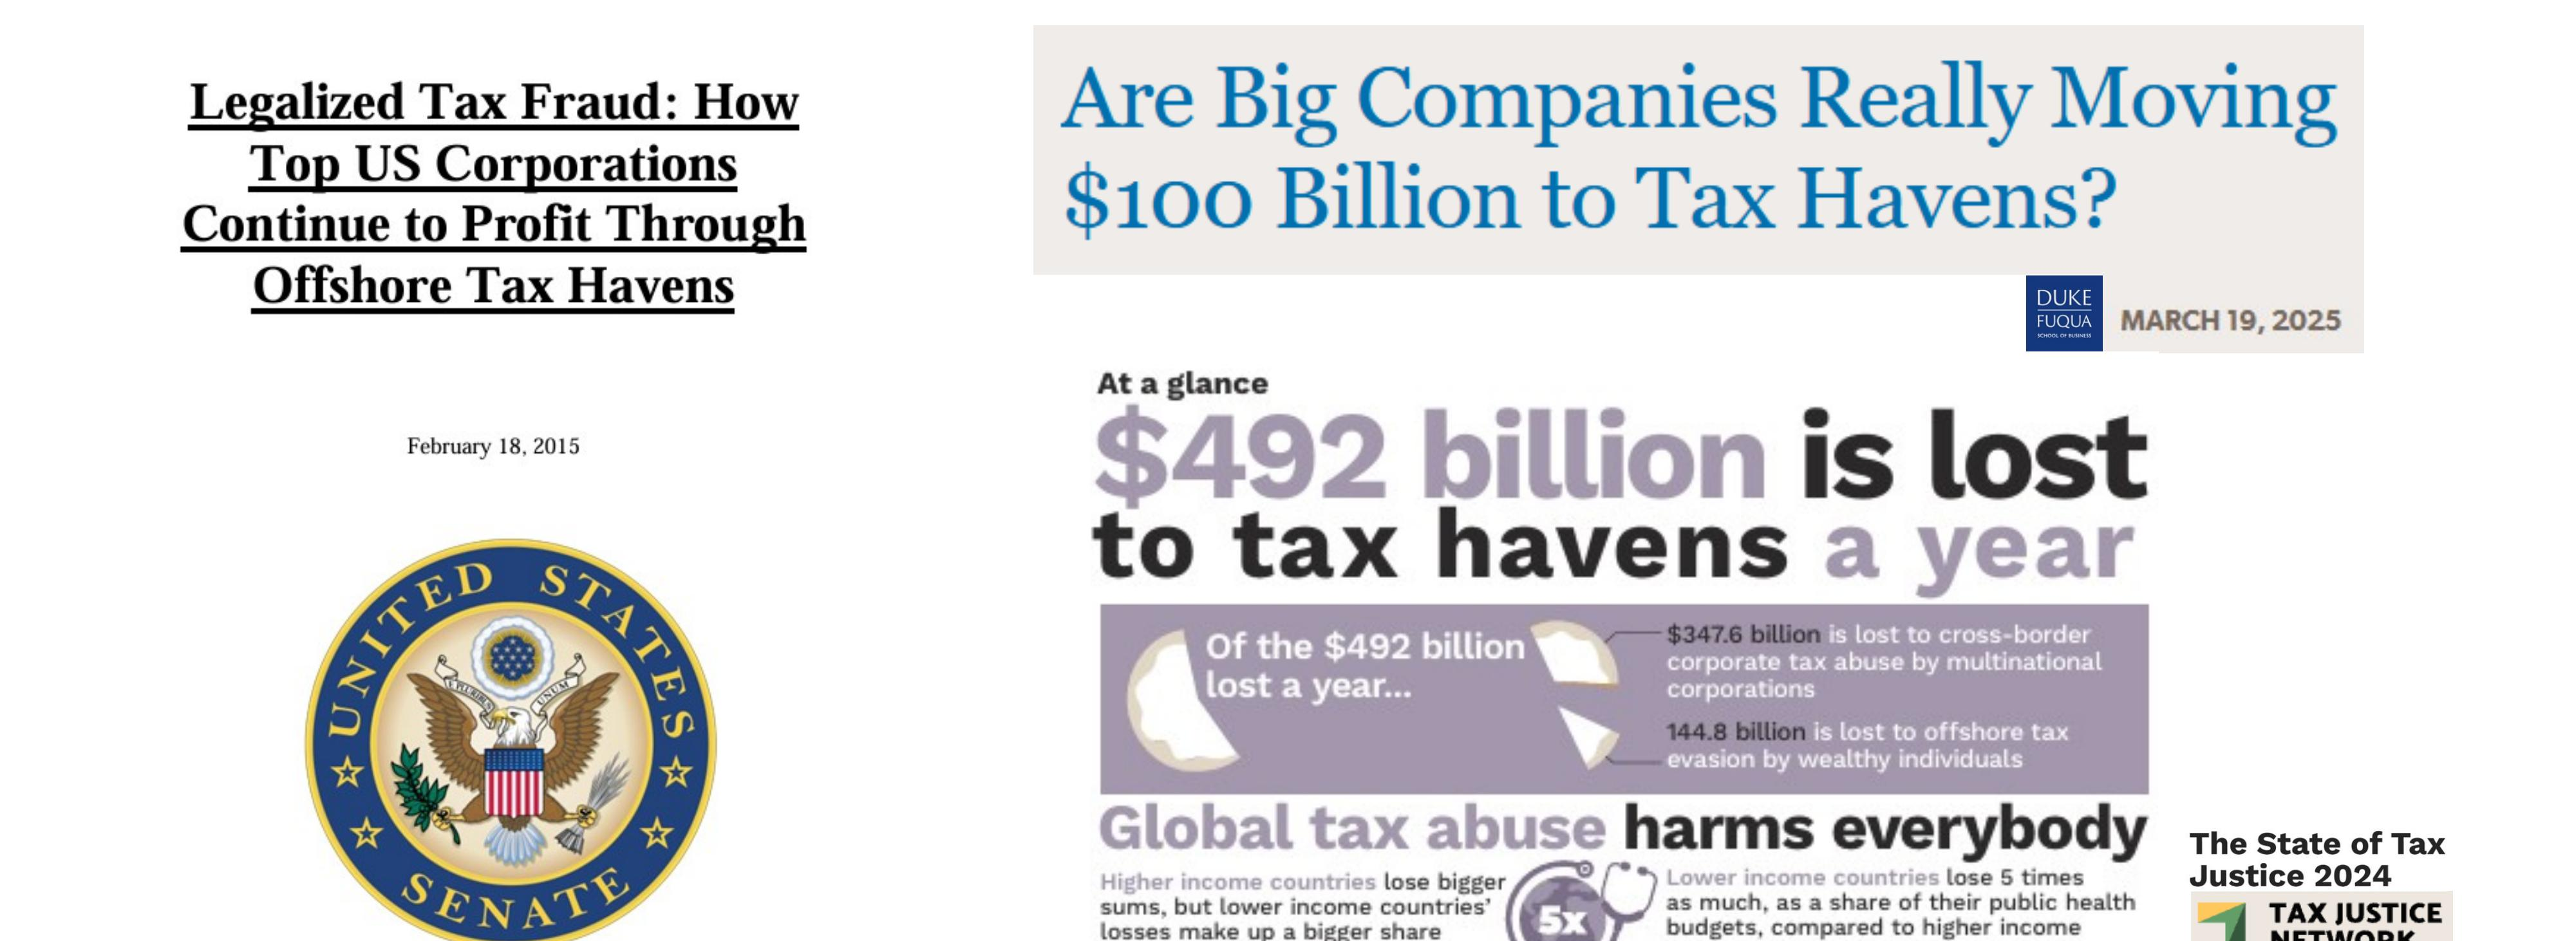
\includegraphics[width=0.95\textwidth, height=0.7\textheight, keepaspectratio]{why_care_slide_cropped.png}
\end{frame}

% ============================================================
% INTRO SLIDE 5: Research Motivation
% ============================================================
\begin{frame}{Introduction -- continued}
\centerline{\large\textbf{Research Motivation}}
\vspace{0.2cm}
Understanding the drivers of income shifting is the key to constructing productive tax incentives which will influence the critical tradeoff between:

\vspace{0.3cm}
\begin{columns}[T]
\begin{column}{0.45\textwidth}
\begin{block}{Shareholder Value}
Minimizing taxes paid to maximize after-tax profits and shareholder returns.
\end{block}
\end{column}
\begin{column}{0.45\textwidth}
\begin{block}{Tax Responsibility}
Contributing appropriate tax amounts to fund government services and infrastructure.
\end{block}
\end{column}
\end{columns}

\vspace{0.4cm}
This study extends prior work by:
\begin{itemize}
    \item Covering fiscal years \textbf{2010--2024} (excluding 2017)
    \begin{itemize}
        \item Including pre- and post-TCJA periods
    \end{itemize}
\end{itemize}
\end{frame}

% ============================================================
% SLIDE 6: Data (variable definitions table replaces descriptive stats)
% ============================================================
\begin{frame}{Data}
\begin{itemize}
    \item \textbf{Source:} WRDS Compustat (Fundamentals Annual + Geographic Segments)
    \begin{itemize}
        \item Publicly traded U.S.\ multinational companies
    \end{itemize}
    \item \textbf{Sample:} 1,553 firm-year observations from 346 U.S.\ MNEs (2010--2024, excluding 2017)
\end{itemize}

\vspace{0.1cm}
{\footnotesize
\begin{center}
\textbf{Variable Definitions}
\end{center}
\vspace{-0.3cm}
\begin{table}
\centering
\begin{tabular}{ll}
\toprule
\textbf{Variable} & \textbf{Definition} \\
\midrule
income\_shift & Foreign profit margin $-$ domestic profit margin \\
tax\_diff & Foreign effective tax rate $-$ U.S.\ statutory rate \\
ww\_profit & Worldwide pre-tax income / total revenue \\
size & Natural log of total assets \\
leverage & Total debt / total assets \\
rnd\_intensity & R\&D expense / total revenue \\
ad\_intensity & Advertising expense / total revenue \\
ppe\_intensity & Net PP\&E / total assets \\
year\_trend & Fiscal year $-$ 2010 \\
post\_tcja & $= 1$ if fiscal year $\geq$ 2018, $= 0$ otherwise \\
\bottomrule
\end{tabular}
\end{table}
}
\end{frame}

% ============================================================
% SLIDE 6b: Data - continued (Figure 2: Scatter)
% ============================================================
\begin{frame}{Data -- continued}
\centering
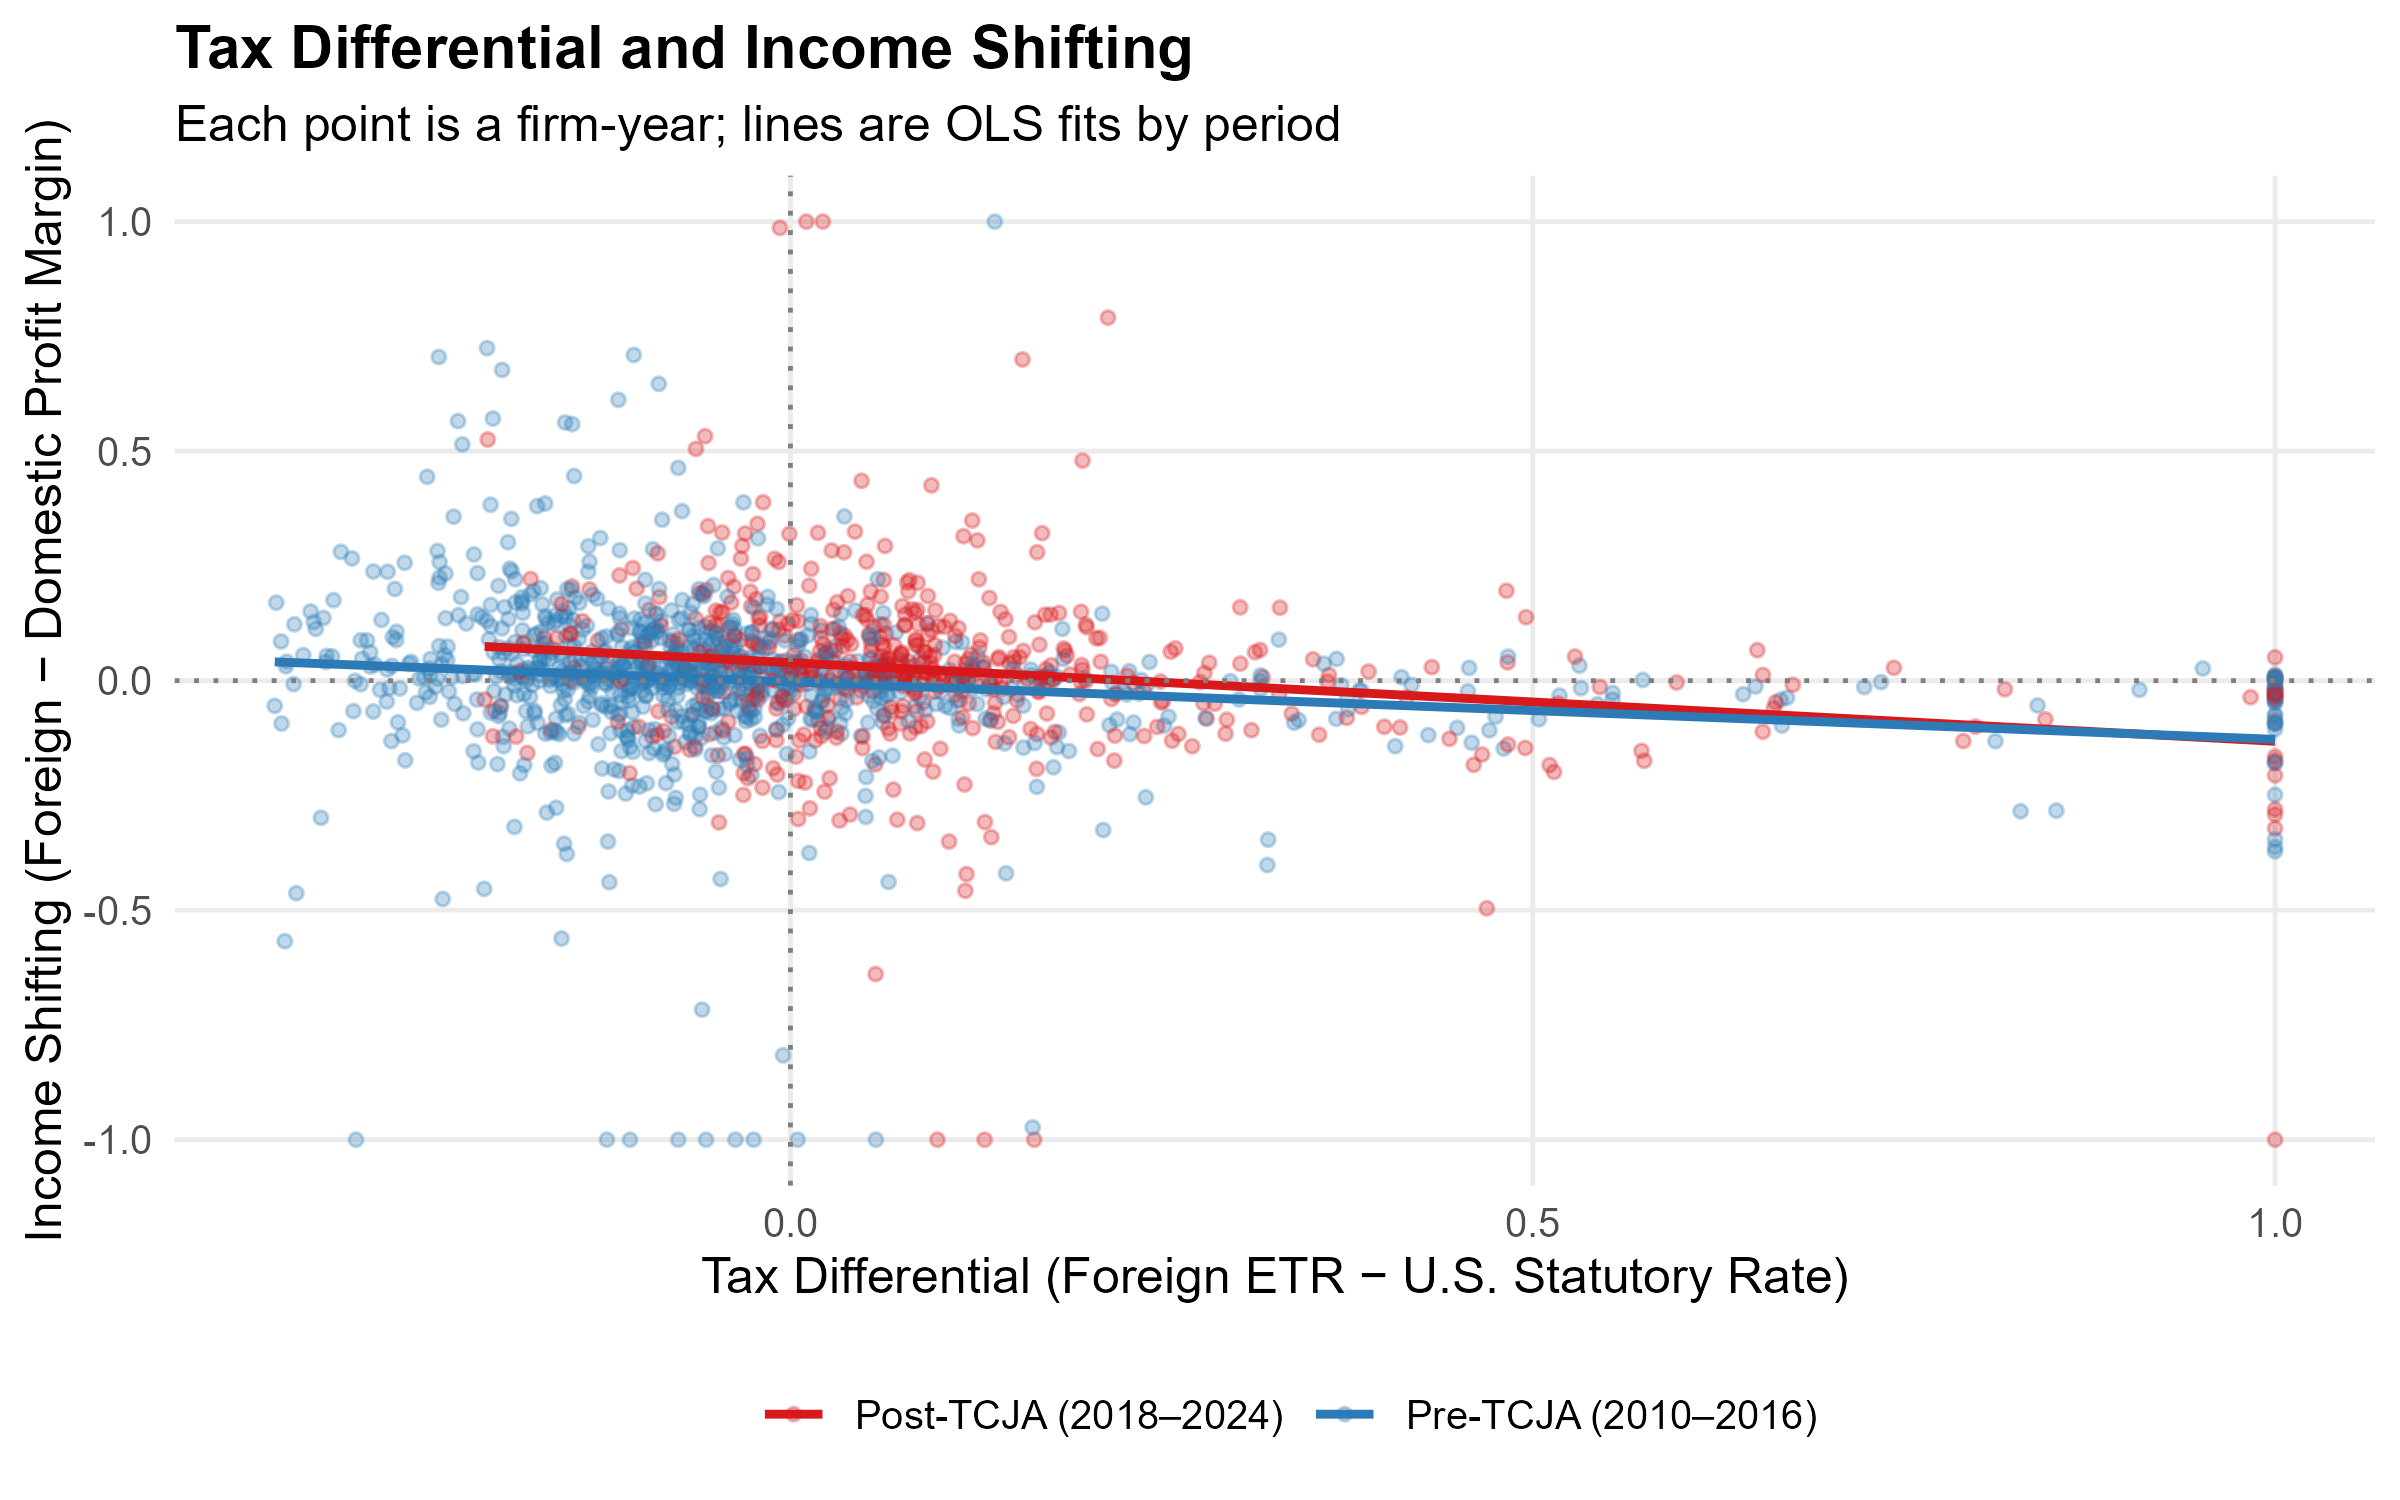
\includegraphics[width=0.85\textwidth, height=0.78\textheight, keepaspectratio]{fig2_tax_diff_vs_shift.png}
\end{frame}

% ============================================================
% SLIDE 6c: Data - continued (Figure 1: Line Chart)
% ============================================================
\begin{frame}{Data -- continued}
\centering
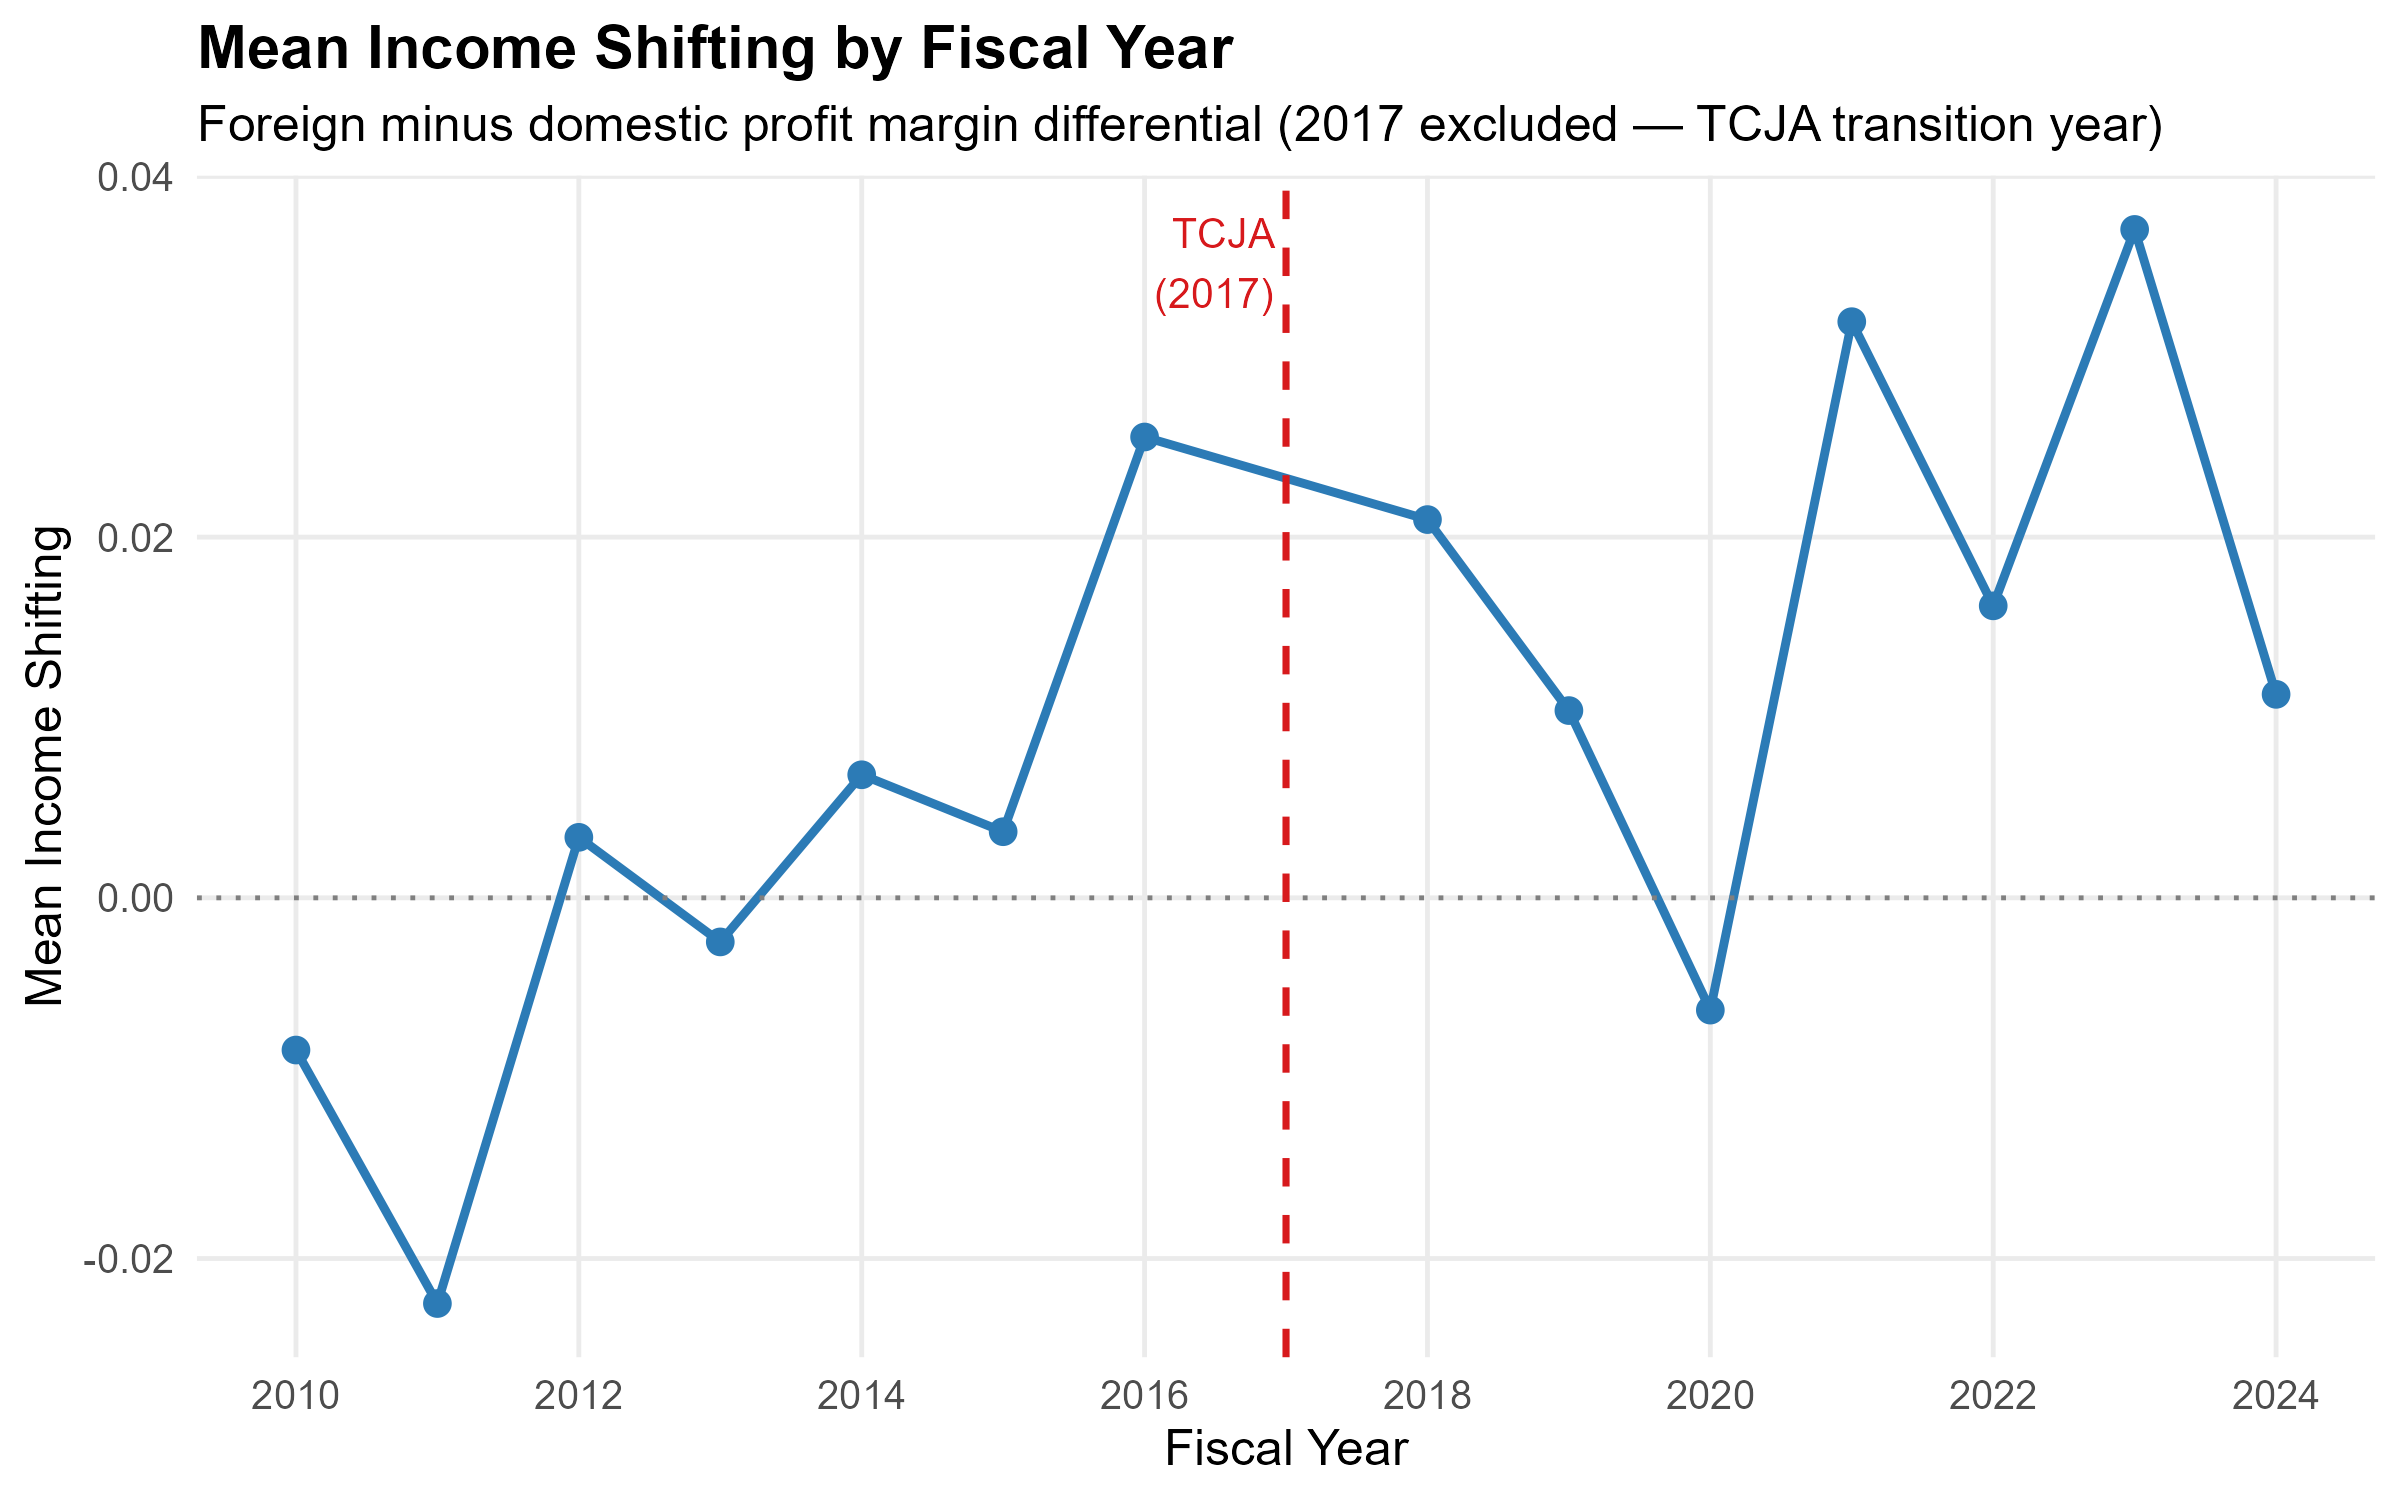
\includegraphics[width=0.85\textwidth, height=0.78\textheight, keepaspectratio]{fig1_income_shift_over_time.png}
\end{frame}

% ============================================================
% SLIDE 6d: Data - continued (Descriptive Statistics - moved here)
% ============================================================
\begin{frame}{Data -- continued}
\centerline{\large\textbf{Descriptive Statistics}}
\vspace{0.2cm}
{\footnotesize
\begin{table}
\centering
\begin{tabular}{lrrrrr}
\toprule
\textbf{Variable} & \textbf{N} & \textbf{Mean} & \textbf{Median} & \textbf{Std Dev} \\
\midrule
income\_shift & 1,553 & 0.0065 & 0.0097 & 0.1802 \\
tax\_diff     & 1,553 & 0.0355 & $-$0.0222 & 0.2512 \\
ww\_profit    & 1,553 & 0.1175 & 0.0970 & 0.0929 \\
size          & 1,553 & 8.2410 & 8.1890 & 1.8920 \\
leverage      & 1,553 & 0.2870 & 0.2520 & 0.2210 \\
rnd\_intensity & 1,553 & 0.0310 & 0.0060 & 0.0590 \\
ad\_intensity  & 1,553 & 0.0120 & 0.0000 & 0.0330 \\
ppe\_intensity & 1,553 & 0.2100 & 0.1380 & 0.2040 \\
\bottomrule
\end{tabular}
\end{table}
}
\end{frame}

% ============================================================
% SLIDE 7: Methods
% ============================================================
\begin{frame}{Empirical Methods}
\textbf{Regression Equation:}
\begin{equation*}
\text{income\_shift}_{it} = \beta_0 + \beta_1 \text{tax\_diff}_{it} + \beta_2 \text{ww\_profit}_{it} + \boldsymbol{\beta} \mathbf{X}_{it} + \varepsilon_{it}
\end{equation*}

\vspace{0.1cm}
\textbf{Progressive specifications:}
\begin{itemize}
    \item \textbf{Model 1:} Baseline with all controls (robust SEs)
    \item \textbf{Model 2:} Year fixed effects
    \item \textbf{Model 3:} TCJA interaction terms
    \item \textbf{Model 4:} Industry (2-digit SIC) fixed effects
\end{itemize}

\vspace{0.2cm}
\textbf{Controls ($\mathbf{X}_{it}$):} firm size, leverage, R\&D intensity, advertising intensity, PPE intensity, year trend, post-TCJA indicator

\vspace{0.2cm}
\textbf{Sensitivity:} Re-estimated on a restricted sample (995 obs) excluding ambiguous geographic segments
\end{frame}

% ============================================================
% SLIDE 8: Regression Results
% ============================================================
\begin{frame}{Findings}
\centerline{\large\textbf{Regression Results (Model 1)}}
\vspace{0.1cm}
{\footnotesize
\begin{table}
\centering
\begin{tabular}{lrrrr}
\toprule
\textbf{Variable} & \textbf{Estimate} & \textbf{Std Error} & \textbf{t Stat} & \textbf{p-value} \\
\midrule
Intercept       &  0.108 & 0.024 &  4.50 & $<$.0001 \\
tax\_diff       & $-$0.162 & 0.027 & $-$6.00 & $<$.0001 \\
ww\_profit      & $-$0.469 & 0.069 & $-$6.80 & $<$.0001 \\
size            &  0.005 & 0.003 &  1.97 & 0.0488 \\
leverage        &  0.086 & 0.022 &  3.91 & $<$.0001 \\
rnd\_intensity  & $-$0.092 & 0.102 & $-$0.90 & 0.3655 \\
ad\_intensity   &  0.231 & 0.092 &  2.51 & 0.0118 \\
ppe\_intensity  &  0.047 & 0.035 &  1.34 & 0.1791 \\
year\_trend     &  0.002 & 0.002 &  1.03 & 0.3018 \\
post\_tcja      &  0.017 & 0.018 &  0.94 & 0.3473 \\
\midrule
\multicolumn{2}{l}{$F = 23.41$, $p < .0001$} & \multicolumn{3}{r}{Adj.\ $R^2 = 11.61\%$, $N = 1{,}536$} \\
\bottomrule
\end{tabular}
\end{table}
}
\end{frame}

% ============================================================
% SLIDE 9: Key Findings
% ============================================================
\begin{frame}{Findings -- continued}
\centerline{\large\textbf{Key Findings}}
\vspace{0.2cm}
{\small
\textbf{Tax Differential} ($\beta = -0.162$, $p < .0001$): \\
Higher foreign tax rates are associated with less outward income shifting. This is consistent with profit-maximizing behavior under the TCJA's reduced U.S.\ rate.

\vspace{0.2cm}
\textbf{Worldwide Profitability} ($\beta = -0.469$, $p < .0001$): \\
More profitable firms shift less income abroad, suggesting these firms face greater scrutiny or have less incentive to shift.

\vspace{0.2cm}
\textbf{Leverage} ($\beta = 0.086$, $p < .0001$): \\
More leveraged firms shift more income, suggesting firms use debt financing and transfer pricing simultaneously as tax strategies.

\vspace{0.2cm}
\textbf{Firm Size} ($\beta = 0.005$, $p = .049$): \\
Larger firms engage in marginally more shifting, consistent with having the resources and infrastructure to do so.

\vspace{0.2cm}
\textbf{Other Controls:} R\&D intensity, PPE intensity, year trend, and post-TCJA indicator are not statistically significant.
}
\end{frame}

% ============================================================
% SLIDE 10: Takeaway / Conclusion
% ============================================================
\begin{frame}{What Did We Learn?}
\begin{itemize}
    \item Tax differentials are the \textbf{strongest driver} of income shifting --- a 1 pp increase in the foreign-domestic tax gap reduces outward shifting by 0.16 pp
    \item Results are robust across year fixed effects, TCJA interactions, industry fixed effects, and a restricted sensitivity sample
    \item Post-TCJA coefficient is insignificant --- \textbf{no clear evidence the reform reduced shifting}
\end{itemize}

\vspace{0.3cm}
\begin{block}{Policy Implication}
Statutory rate cuts alone may not curb profit shifting. Other tax rules or incentives should be considered including different enforcement.
\end{block}

\vspace{0.2cm}
\textbf{Limitations:} Compustat geographic segments may not capture all shifting channels; excludes financial firms
\end{frame}

% ============================================================
% FINAL SLIDE: Thank You
% ============================================================
\begin{frame}
\centering
\vspace{1.5cm}
{\Huge\textbf{Thank You!}}

\vspace{1cm}
{\Large Any Questions?}
\end{frame}

\end{document}
